\documentclass[letter, 11pt]{article}
\usepackage[utf8]{inputenc}
\usepackage{amsmath}
\usepackage{amsfonts,txfonts}
\usepackage{mathrsfs}
\usepackage[colorlinks, urlcolor=blue]{hyperref}
\usepackage{fourier}
\usepackage[top = 2.5cm, bottom = 2cm, left = 2cm, right = 2cm]{geometry}
\usepackage{graphicx}
\usepackage{scalerel,stackengine}
\usepackage{indentfirst}


\title{\textsc{First Report: Wavelet Clumps Project} \\
    \textsc{INF491: Astroinformatics}}

\author{Martín Villanueva}
\date{9 june 2016}

\begin{document}
\maketitle





\section{\textsc{Formal Problem Definition}}

In concise words the problem to be addressed consists on given a 3D spectroscopic cube of data (mostly from observations of cold molecular clouds), build an algorithm that automatically can identify clump structures, and determine the hierarchical relationships between them.\\

So in order to see the difficulties of the problem, it's imperative to understand what a clump is. There is some debate about the true nature of clumps, but is generally understood that a clump is an area of high density within a larger area of lower density, in relation to the star formation in molecular clouds. This molecular clouds are usually non homogeneous in their density, and are composed of cores of high density gas matter contained and separated by low density areas. Each observation of such clouds, may contain multiple source cores in a very complex configurations. A few time ago astronomers analyzed these images manually (by eye), but this is no longer possible because of three major reasons:
\begin{enumerate}
    \item These manual methods doesn't scale as fast as the generation of new data observations, such as those performed by ALMA.
    \item The size of the images is huge and could contain hundreds/thousands of cores (Figure \ref{fig:barnard68}). So it may require a lot of time to analyze it manually.
    \item The results of clump identification performed (manually) by astronomers usually didn't match, because they have different conceptions and notions of what clumps are and how they relate each other.
\end{enumerate}

\begin{figure}[htpb!]
\centering
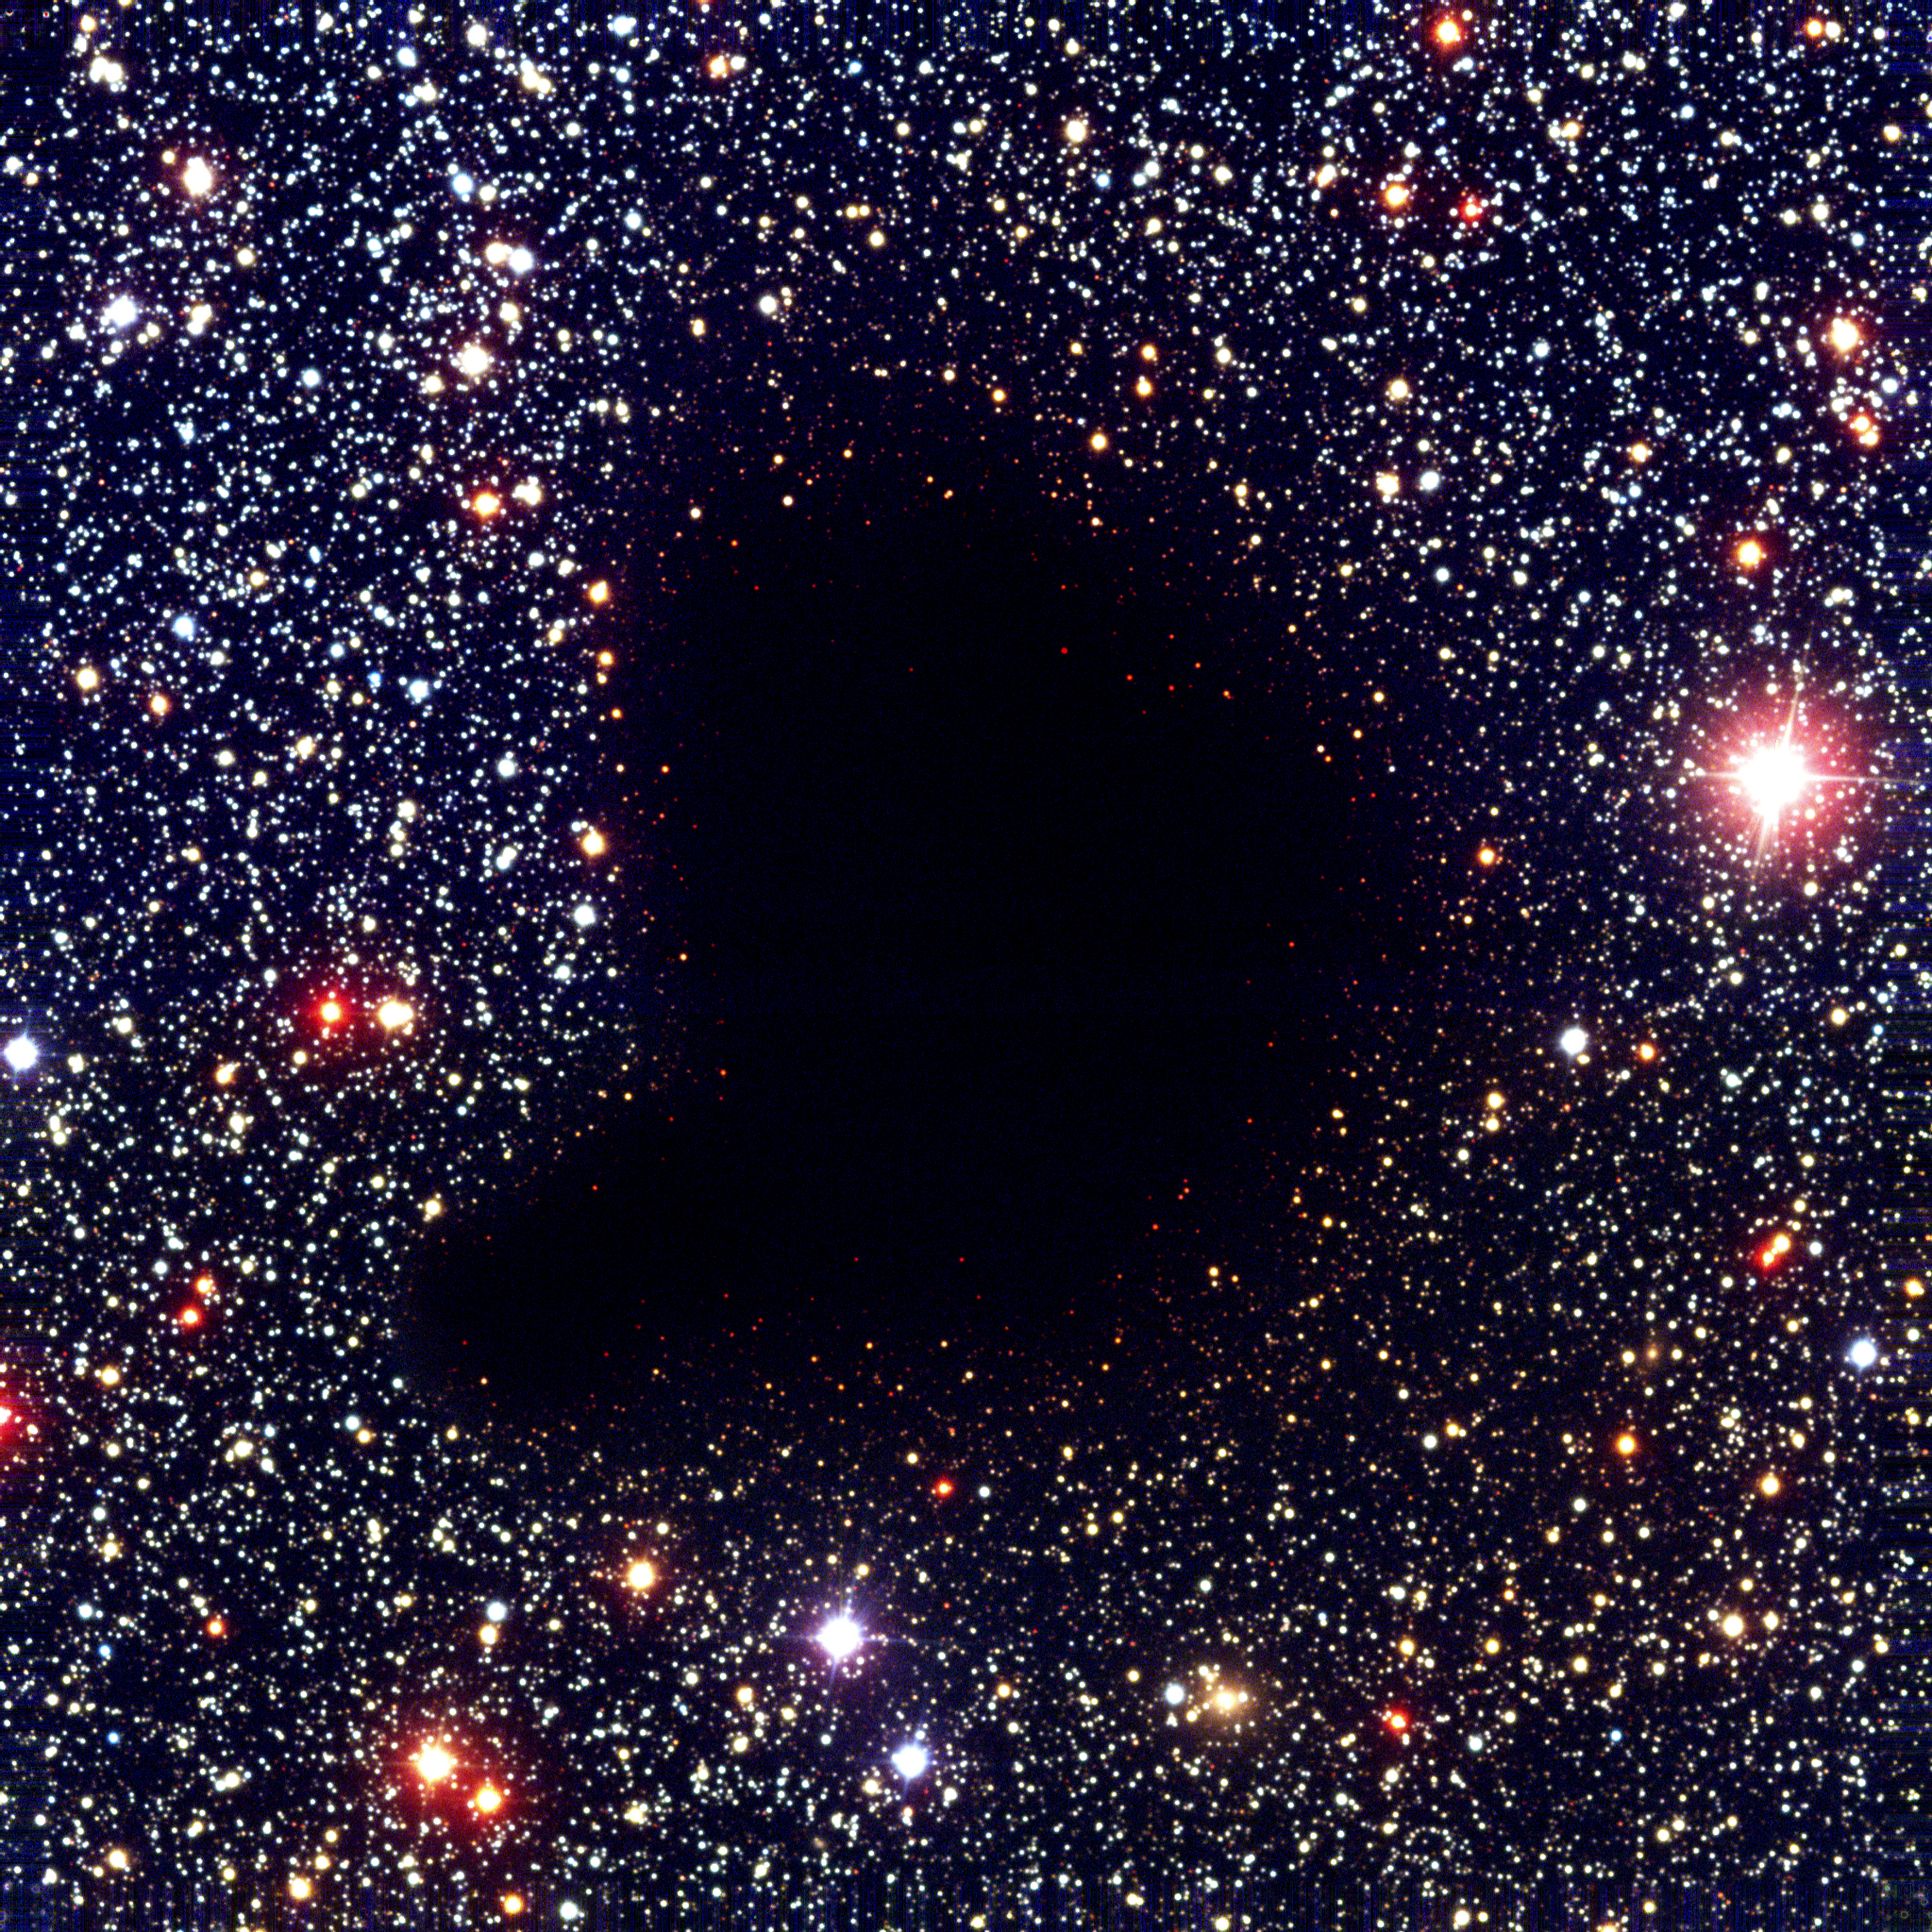
\includegraphics[width=6cm]{barnard68}
\caption{Barnard 68 molecular cloud}
\label{fig:barnard68}
\end{figure}

The third reason is the most important. As the image becomes more crowded with clumps, problems like blended emissions arise, where multiple dense cores converge in a nearby area. In this cases subjective biases become more evident as each astronomer could perceive the data differently. So it will be great if an automated clump detection algorithm could do the job, removing the individual bias and so providing consistent and objective results.\\

Other complications is that 3D spectroscopic cubes (in FITS format) will be used instead of 2D cubes. They have \textit{right ascension}, \text{declination} and \textit{frequency} coordinates with the associated observed intensity. Unlike the 2D version of collapsed cubes (in frequency), it is hard to analyze this kind of data by eye because of the high number of dimensions.\\

The final difficulty is to determine the hierarchical relationships between the found clumps. As explained above, each dense core is often contained on lower density cores, constituting a hierarchical structure. Determining this relations is fundamental to understand processes like the \textit{star formation}. But (again) there isn't a straightforward and unbiased way to do that.

    




\section{\textsc{State of the Art}}

The problems stated in the previous section has been addressed in the last two/three decades with different approaches. Nevertheless, some of these have solved just a piece of the whole problem. In the following, a description will be given about the principal algorithms used to solve the problems of \textit{clump identification} and determining the \textit{hierarchical relation}.

\subsection{\textsc{Clump Identification}}

\begin{description}
    \item[\textbf{GaussClumps.}] This was proposed by Stutzki et al. \cite{Stutzki}, and was the first successful approach to handle the problem of automatically detect clumps. The main idea is to adjust Gaussian profiles that best fits each of the emission peaks. The reason why use Gaussian functions over some other choice, it is because experimental observations of the most abundant molecules on molecular clouds, have shown that his intensity distribution have a shape more or less like Gaussians.  

    The algorithm iteratively searches for the actual emission peak, and tries to fit a Gaussian function (searching for the best parameters of that Gaussian) through a minimization process. Then this Gaussian is subtracted from the data cube, and the same step is repeated over the residual cube. As result we get a set a gaussians with different positions, orientations and intensities. The sum of all this Gaussian components plus the background noise, allows us to recreate the data cube.

    In this algorithm each Gaussian is considered as a single clump, and because Gaussians could overlap between them, then it is possible that pixels are assigned to more than one clump.


    \item[\textbf{ClumpFind.}] This algorithm was developed by Williams et al. \cite{Williams}.  It was motivated by how the human eyes identifies structures on images, i.e, how the eye decomposes the maps into clumps by looking at the contour levels in a gradually and decreasing way. So the algorithm works by contouring the data at multiples of the rms noise of the observations. It starts from the highest level, where isolate cores are identified and each of these is considered as new clump. Then this step is repeated by gradually decreasing the level where to search,  identifying isolate structures and connecting them with clumps identified at previous levels, or defining them as new clumps otherwise. When a clump identified at a given level touches more than one clump identified at a previous level, then this structure correspond to a blended emission, and should be splitted. To do that a \textit{friends-of-friends} strategy is used, assigning each pixel of the identified structure to one of the adjoining clumps (\textit{with more friends}).

    As result of this process a \textit{Clump Assignment Array} structure is generated, where each pixel is assigned exclusively to one clump, as shown in Figure \ref{fig:cf}. A key characteristic of ClumpFind is that no a priori clump profile is assumed, and then the identified clumps can have any shape.
    \begin{figure}[htpb!]
    \centering
    \includegraphics[width=6cm]{cf}
    \caption{ClumpFind results on 2D data (Source: \cite{Williams})}
    \label{fig:cf}
    \end{figure}

    \item[\textbf{FellWalker.}] A totaly different approach was proposed by Berry \cite{Berry}, in which a gradient-tracing scheme similar to \textit{Hill-Climbing} it is used in order to reach a local emission peak, which defines a new clump. FellWalker like ClumpFind, segments the supplied data cube into a number of disjoint regions, each associated with a single significant peak.

    The algorithms works by computing ascent paths (with the highest gradient) for each single pixel (Figure \ref{fig:fw}). These paths have two alternatives: 1) Reach a local peak and so find a new clump (in that case a new search it's performed on a wider neighborhood to verify that it is really a peak). 2) Reach another ascent path computed previously, and so assign the pixels on that path to the corresponding (crashed) clump. At the end of the algorithm, detected clumps with low dip between them, are merged as a single clump.
    \begin{figure}[htpb!]
    \centering
    \includegraphics[width=6cm]{fw}
    \caption{Two ascent paths of FellWalker on 2D data (Source: \cite{Berry})}
    \label{fig:fw}
    \end{figure}

\end{description}

\subsection{\textsc{Hierarchical Relations}}

\begin{description}
    \item[\textsc{Dendrograms.}] Dendrograms approach was proposed by Rosolowsky et al. \cite{Rosolowsky}. This method is philosophically different from local segmentation algorithms like ClumpFind or FellWalker, since it points to track the hierarchical structure over a range of scales. Similar to ClumpFind, this algorithm computes the isosurfaces for molecular data cubes, representing the hierarchical structure of these, in a tree data-structure also know as Dendrograms. Points in the dendrogram structure correspond to specific volumes in data cubes, defined by their bounding
    isosurfaces.

    If the ClumpFind algorithm divides a contour map in pieces of a puzzle, then the Dendrograms try to divide that puzzle in a collection of different layers that represents the cores. The order and structure of the tree, defines the physical relations between the identified cores.

    \item[\textsc{Multiresolution Analysis.}] Multiresolution Analysis (MRA) it is a technique widely used in the last years to analyze astronomical data images. In particular one of the major tools to perform MRA is the Wavelet Transform, which maps input data to the \textit{scale-position} Wavelet space. As explained by Starck \cite{Starck}, \textit{Discrete Wavelet Transform} (DWT) can be used to transform the data and see it with different resolutions, i.e, have a view of the data with different levels of details, and then we can see fine-grained to coarse-grained details. A very useful type of DWT is the \textit{Stationary Wavelet Transform} (SWT), also called \textit{À trous} wavelet transform. This consist on a redundant version of DWT, that has the property of mapping input images to images in the wavelet space with the same size (because of the redundancy). Because of that, all the analysis could be done at the Wavelet space.

    In his study of the stellar \textit{Initial Mass Function} (IMF), Alves et al. \cite{Alves} applied the SWT to images of interstellar molecular clouds, in order to have a detailed knowledge of the spectrum of masses of dense cores. The clump identification procedure first map the corresponding (2D) image, to the wavelet space at different scales. For a given scale $i$, structures are isolated at $3\sigma_i$, with $\sigma_i$ being the noise of the image at scale $i$. Then a detected structure at scale $i$ is connected with a structure at scale $i+1$ if its local maxima drops in the structure at scale $i+1$.

    On the other side Gregorio et al. \cite{Gregorio} follows a very similar approach, performing SWT over 2D images to get a multiresolution view of the data. However, he wasn't satisfied with the thresholding step of above, guessing that applying threshold isn't a good way of segmenting the data. Instead he proposed to use clump identification algorithms (like ClumpFind), to segment the data at the different levels on the Wavelet space. The results of such procedure are shown in Figure \ref{fig:greg}.
    \begin{figure}[htpb!]
    \centering
    \includegraphics[width=12cm]{greg}
    \caption{Clump Identification at 4 different scales on Wavelet Space (Source: \cite{Gregorio})}
    \label{fig:greg}
    \end{figure}
    Applying the same criterions as Alves \cite{Alves}, a hierarchical relation could be stated between the structures found at the different scales, to create a Dendrogram like structure.
\end{description}




\newpage
\section{\textsc{Proposed Solution}}
In order to solve the problem of identification and hierarchical relation of clumps on spectroscopic data cubes, it is proposed to extend the ideas of Alves \cite{Alves} and Gregorio \cite{Gregorio}, but to 3D data cubes. Then MRA will be required over the 3D data cube, i.e, a 3D discrete Wavelet transform should be applied to extract the features at different scales. After computing the 3D DWT, the procedure continues similarly to the previous; A clump identification/segmentation algorithm is applied to each new cube, and then the results of the different levels are summarized in a Dendrogram tree structure. An outline of this procedure is shown on Figure \ref{fig:wavclump}.
\begin{figure}[htpb!]
\centering
\includegraphics[width=12cm]{wavclump}
\caption{Proposed Solution Outline}
\label{fig:wavclump}
\end{figure}
However, some considerations must be taken into account:
\begin{enumerate}
    \item As explained previously, the SWT maps input images to images in the Wavelet space with the same size. So if we are working with huge 3D data cubes, the process of computing the SWT for each level will require a considerable computing time and memory allocation. Additionally, there isn't nowadays any software package that implements the 3D version of the SWT.
    \item Then the possibilities are to adapt somehow the SWT, or make use of the standard DWT (\textit{which work on N-dimensional data}. The last one maps the input image to a sparse representation on the Wavelet space, and then there isn't longer possible to work directly on this space. An option is to compute the Inverse Discrete Wavelet Transform (IDWT), and taking this like the MRA representation.
    \item In order to get coherent results, a 3D wavelet has to be chosen (or constructed) so that features computed at the different levels are useful.
\end{enumerate}

Additionally this solutions propose to take an intermediate point between Alves and Gregorio Identification/Segmentation step. Images on a low level (in the Wavelet space) have fine-grained details, and so they need a robust algorithm to perform the segmentation step. On the other hand, images with a high level have coarse-grained details, and so they don't need a complex algorithm to segment it, probably with just a thresholding the segmentation will be good enough. Then it is possible to take the good things of both approaches. In that way, the whole process could be optimized by performing robust (and computationally expensive) methods on data with fine-grained details, and performing some simpler methods (and computationally cheap) on data with coarse-grained details.

To perform fast segmentation there are many methods: Simple thresholding, adaptive thresholding, watershed algorithm, and many more from the computer vision and image processing fields.


\section{\textsc{Concept Tests}}

In the following concept test, a FITS image of Orion Methanol observations is used, with $41$ channels of frequency. In order to visualize the data, four slices at $freq=8,\ 16,\ 24,\ 32$ are shown (Figure \ref{fig:level0}).
\begin{figure}[htpb!]
\centering
\includegraphics[width=14cm]{level0}
\caption{Original slices}
\label{fig:level0}
\end{figure}

To perform the multiresolution analysis, a 3D DWT is used with a Haar Wavelet. The first three levels are obtained by sequentially computing the low-pass (approximation) coefficients and the high-pass (details) coefficients. The results of the reconstruction process are shown in figures \ref{fig:level1}, \ref{fig:level2} and \ref{fig:level3} respectively.

\begin{figure}[htpb!]
\centering
\includegraphics[width=14cm]{level1}
\caption{Slice at level 1}
\label{fig:level1}
\end{figure}

\begin{figure}[htpb!]
\centering
\includegraphics[width=14cm]{level2}
\caption{Slices at level 2}
\label{fig:level2}
\end{figure}

\begin{figure}[htpb!]
\centering
\includegraphics[width=14cm]{level3}
\caption{Slices at level 3}
\label{fig:level3}
\end{figure}

Then can be noted that as the level gets higher, less detailed data we get, i.e, the coarse-grained details are appearing. As stated in the \textit{Proposed Solution} section, it is clear that in the high levels the clump structures are much more easy to identify that the ones in lower levels.

In order to verify the last point, a thresholding procedure similar to Alves \cite{Alves} was performed on data at level $1$ and $3$, which can be seen in Figures \ref{fig:th1} and \ref{fig:th3} respectively.
\begin{figure}[htpb!]
\centering
\includegraphics[width=14cm]{threshold1}
\caption{Thresholding slices at level 1}
\label{fig:th1}
\end{figure}

\begin{figure}[htpb!]
\centering
\includegraphics[width=14cm]{threshold2}
\caption{Thresholding slices at level 3}
\label{fig:th3}
\end{figure}
Thresholding the coarse-grained data gives very good results, getting almost the exact clump structure. On the other hand, thresholding the fine-grained data gives poor results, detecting regions that are not actually part of cores.

\newpage
\bibliography{references}{}
\bibliographystyle{plain}

\end{document}